\documentclass[11pt,letterpaper]{article}
\usepackage[T1]{fontenc}
\usepackage{lmodern,microtype,amsmath,booktabs,graphicx,caption,xcolor,hyperref}
\usepackage[margin=0.95in]{geometry}
\usepackage{float}

\definecolor{ink}{HTML}{253D56}
\hypersetup{colorlinks=true,allcolors=ink,
  pdftitle={Lexical and Dense Passage Retrieval on MS MARCO},
  pdfauthor={Aritro}}
\captionsetup{font=small,labelfont=bf,labelsep=period,skip=5pt}
\setlength{\dblfloatsep}{8pt}
\setlength{\floatsep}{8pt}
\setlength{\intextsep}{8pt}
\setlength{\textfloatsep}{10pt}

\setlength{\parindent}{0pt}
\setlength{\parskip}{6pt plus 1pt}
\setlength{\tabcolsep}{4pt}
\renewcommand{\arraystretch}{1.10}
\raggedbottom

\title{\bfseries Lexical and Dense Passage Retrieval\\on MS MARCO}
\author{Aritro \\ \small NYU Tandon School of Engineering}
\date{\small CS 6913 \enspace $\cdot$ \enspace Assignment 3}

\begin{document}
\maketitle

\begin{abstract}
We compare BM25, FAISS HNSW, and BM25 with embedding reranking on the same one million MS MARCO passages. Reranking led on all reported quality metrics on TREC 2019 and MS MARCO dev. HNSW led on Recall@100 and both NDCG cutoffs on TREC 2020. In three 43-query batch trials, HNSW had the shortest median wall time and BM25 used the least query memory. Reordering only the first 10 to 100 BM25 hits improved the mean of every metric examined in the depth sweep.
\end{abstract}


\section{Introduction}
We ask how much passage ranking improves when dense scores are available and what that improvement costs. We compare lexical retrieval, direct dense retrieval, and dense reranking of lexical candidates on the same collection. We also vary the reranking depth and examine whether retrieval quality changes with query length.
\section{Collection and retrieval systems}
We filtered the original passage collection by the supplied IDs and rebuilt the compressed Rust BM25 index on the resulting one million passages. The supplied passage and query embeddings have 384 dimensions. Every system returns original MS MARCO passage IDs.

\textbf{BM25.} The engine scores passages that contain any normalized query term, with $k_1=1.2$ and $b=0.75$ \cite{bm25}. The PS3 batch mode opens the index once, disables snippets, and saves up to 1,000 hits per query. The vector scripts use the same output fields so the evaluator can read all three runs.

\textbf{HNSW.} FAISS \texttt{IndexHNSWFlat} searches the full subset by raw inner product \cite{hnsw,faiss}. The build converts passage vectors from float16 to float32 and associates each vector with its passage ID. The graph uses $M=8$ and \texttt{efConstruction}=100. Search uses \texttt{efSearch}=200 and requests up to 1,000 hits.

\textbf{BM25 reranking.} We compute the raw dot product between the query embedding and each BM25 candidate, then sort in descending score order. A stable sort keeps BM25 order for equal scores. The main comparison reranks all available candidates up to 1,000.


\newpage
\subsection{Design decisions}
The three systems exchange rankings in the same four-column format: query ID, passage ID, rank, and score. Each row keeps the original MS MARCO identifiers. BM25 and the vector methods compute different kinds of scores, so evaluation uses the saved rank and joins it to judgments by query and passage ID. This lets one evaluator handle all three methods, including queries with no returned hits.

\subsubsection*{Lexical retrieval and the candidate list}
We retained the Rust BM25 scorer from PS2 and added batch input and configurable result depth for PS3. The tokenizer splits at non-alphanumeric characters and lowercases the tokens. In OR mode, a passage can enter the candidate list if it contains any query term. The index is loaded once per batch, and snippets are disabled because the evaluation needs the ordered passage IDs. The scorer returns up to 1,000 hits. This gives the reranker a pool deeper than the evaluation cutoffs at 10 and 100.

\subsubsection*{Building and searching the dense index}
HNSW navigates a graph to find high-scoring passage vectors approximately \cite{hnsw}. The parameter \(M\) controls graph connectivity. \texttt{efConstruction} controls candidate exploration when adding vectors, and \texttt{efSearch} controls exploration during search. We used the single configuration \(M=8\), \texttt{efConstruction}=100, and \texttt{efSearch}=200 in the experiments. These settings determine the graph we timed and the search effort behind the reported quality. The measured results describe this configuration.

The builder reads 25,000 passage embeddings at a time and converts each batch from float16 to float32 before inserting it. FAISS keeps the vectors in the index and uses an ID map to translate search hits to their original passage IDs. We save the graph and its vectors to \texttt{hnsw.faiss}. The search script reloads this index and reads query embeddings in batches of up to 64. The build batch size limits how many input vectors are converted at once. The search batch size controls how many queries are submitted together.

\subsubsection*{Scoring a fixed candidate list}
Reranking reads BM25's output for one query at a time. It maps each candidate passage ID to a row of the passage embedding array and computes an exact dot product within this list. Both dense methods use raw inner product to match the supplied embeddings. The reranker keeps the supplied arrays in float16 and converts the current query and candidate vectors to float32 for scoring. The stable sort preserves the original BM25 order for ties. In the cutoff sweep, the passages below rank \(k\) stay in their BM25 order so changes can be attributed to the reranked portion of the list.

\newpage
\section{Evaluation protocol}
We selected queries by ID from the judgments and used their text for BM25 and their embeddings for the vector methods. TREC 2019 (\texttt{eval.one}), TREC 2020 (\texttt{eval.two}), and MS MARCO dev (\texttt{dev}) have 43, 54, and 1,000 judged queries. All nine runs covered every judged query. Three dev queries returned fewer than 1,000 BM25 candidates.

TREC grades 2 and 3 count as relevant for MRR@10 and Recall@100 \cite{trec19,trec20}. Dev uses label 1. Reciprocal rank gives \(1/r\) for the first relevant hit at rank \(r \le 10\), with zero otherwise. Recall@100 counts the share of known relevant passages found in the first 100. NDCG uses the original grades as linear gains and normalizes against an ideal ranking at the same cutoff. On dev, average precision sums precision at each relevant hit and divides by the total number of known relevant passages. MAP averages that score across queries. Each query has equal weight and unjudged passages contribute zero gain.

\begin{table}[H]
\centering\small
\caption{Quality on the two graded TREC splits.}
\label{tab:trec}
\begin{tabular}{@{}lrrrr@{}}
\toprule
System & MRR@10 & Recall@100 & NDCG@10 & NDCG@100\\
\midrule
\multicolumn{5}{@{}l}{\textit{TREC 2019 (43 queries)}}\\
BM25 & .5923 & .5525 & .4497 & .5322\\
HNSW & .8050 & .6209 & .6777 & .6425\\
BM25 reranked & \textbf{.8283} & \textbf{.6452} & \textbf{.7027} & \textbf{.6620}\\
\addlinespace[3pt]
\multicolumn{5}{@{}l}{\textit{TREC 2020 (54 queries)}}\\
BM25 & .6290 & .6179 & .4912 & .5123\\
HNSW & .7797 & \textbf{.7356} & \textbf{.6632} & \textbf{.6397}\\
BM25 reranked & \textbf{.7817} & .7105 & .6578 & .6331\\
\bottomrule
\end{tabular}
\end{table}

\begin{table}[H]
\centering\small
\caption{Quality on MS MARCO dev (1,000 queries).}
\label{tab:dev}
\begin{tabular}{@{}lrrr@{}}
\toprule
System & MRR@10 & Recall@100 & MAP\\
\midrule
BM25 & .3940 & .7960 & .3967\\
HNSW & .5512 & .8732 & .5494\\
BM25 reranked & \textbf{.5783} & \textbf{.8873} & \textbf{.5755}\\
\bottomrule
\end{tabular}
\end{table}


The graded and binary measures answer different questions. A TREC passage graded 1 can increase NDCG if it moves up, while it contributes zero to recall and reciprocal rank. A passage that moves from rank 11 to rank 9 can improve NDCG@10 and, if it is the first highly relevant hit, MRR@10. Its move leaves Recall@100 unchanged because both ranks are inside that cutoff. These differences explain why the tables report several metrics for each run.

\newpage
\section{Retrieval quality}
\textbf{TREC 2019.} Reranking improved NDCG@10 from 0.4497 to 0.7027 and led HNSW on all four measures in Table~\ref{tab:trec}. The higher NDCG@10 and NDCG@100 show gains in graded ordering at both depths. The 0.0927 increase in Recall@100 over BM25 came from reordering a fixed candidate set. More judged relevant passages reached the first 100 even though both systems retrieved the same candidates at full run depth.

\textbf{TREC 2020.} HNSW led on Recall@100 and both NDCG cutoffs. Its Recall@100 was 0.7356, compared with 0.7105 for reranking. Reranking had the higher MRR@10 by 0.0020. MRR depends on the first relevant passage and can improve even when the rest of the top 100 contains fewer relevant passages. The difference in MRR is small on 54 queries and we did not test statistical significance.

\textbf{MS MARCO dev.} Reranking led all three measures in Table~\ref{tab:dev}. MAP rose from 0.3967 for BM25 to 0.5494 for HNSW and 0.5755 for reranking. The reranking gain over BM25 on MAP (0.1788) was larger than its gain on Recall@100 (0.0913). MAP rewards moving relevant passages earlier, while recall at a fixed cutoff changes only when a relevant passage crosses that cutoff.

\subsection{How often individual queries improved}
Table~\ref{tab:paired} counts how often MRR@10 improved, tied, or declined relative to BM25. On dev, HNSW improved five more queries than reranking did, yet reranking had the higher mean. Reranking also lowered MRR@10 on fewer queries. The mean is sensitive to the size of a change as well as its direction. Moving the first relevant hit from rank 2 to rank 1 adds 0.5, while moving it from rank 10 to rank 9 adds about 0.011.

\begin{table}[H]
\centering
\caption{Per-query changes in reciprocal rank at 10 relative to BM25.}
\label{tab:paired}
\begin{tabular}{llrrr}
\toprule
Split & System & Improved & Tied & Declined\\
\midrule
TREC 2019 & HNSW & 19 & 19 & 5\\
          & BM25 reranked & 19 & 20 & 4\\
TREC 2020 & HNSW & 21 & 25 & 8\\
          & BM25 reranked & 21 & 25 & 8\\
Dev       & HNSW & 447 & 377 & 176\\
          & BM25 reranked & 442 & 424 & 134\\
\bottomrule
\end{tabular}
\end{table}

\subsection{The candidate pool limits reranking}
If the BM25 candidates were ordered with perfect knowledge of the judgments, mean Recall@100 would reach at most 0.7807 on TREC 2019, 0.8323 on TREC 2020, and 0.9082 on dev. For each query, this bound counts the relevant passages in the BM25 candidate set, caps the count at 100, and divides by the known relevant total. On TREC 2020 the bound of 0.8323 exceeds both the actual reranked score of 0.7105 and the HNSW score of 0.7356. The candidate restriction alone cannot explain HNSW's lead. The ordering within the BM25 pool also leaves room for improvement.

\newpage
\subsection{Which relevant passages the systems recover}
Mean recall gives each query equal weight. To see where the rankings differ, we also counted judged relevant query--passage pairs in the first 100 results of HNSW and reranking. A passage contributes once per query, so the same passage can contribute again for another query. We applied the same binary relevance thresholds as in Recall@100. Table~\ref{tab:overlap} reports counts summed over queries. Queries with more judgments can therefore contribute more pairs to this table.

\begin{table}[H]
\centering\small
\caption{Judged relevant pairs in the top 100 of HNSW and BM25 reranking. The last column counts HNSW hits outside the full BM25 candidate list.}
\label{tab:overlap}
\begin{tabular}{@{}lrrrr@{}}
\toprule
Split & Both & HNSW only & Reranker only & Outside BM25\\
\midrule
TREC 2019 & 1,030 & 117 & 142 & 117\\
TREC 2020 & 792 & 94 & 46 & 93\\
MS MARCO dev & 865 & 68 & 82 & 68\\
\bottomrule
\end{tabular}
\end{table}

\textbf{Coverage beyond lexical candidates.} On TREC 2020, 93 of the 94 relevant pairs unique to the HNSW top 100 were outside the full BM25 candidate list. Those 93 pairs came from 20 of the 54 queries. No ordering of those particular BM25 lists could recover these hits. At the same time, the reranker placed 46 pairs in the top 100 that HNSW did not return there. Direct dense retrieval and lexical candidate selection followed by dense scoring recovered overlapping sets with distinct contributions.

\textbf{Why coverage and order both matter.} On TREC 2019, HNSW found 117 relevant pairs outside the BM25 pool, yet reranking had the higher mean Recall@100. Within the two top-100 rankings, the reranker contributed 142 unique pairs. This illustrates why access to the full collection is only one part of the comparison. A system still has to rank the relevant hits it finds high enough to count. The BM25 candidate ceiling in the previous section shows how much room remains for a better ordering within that pool.

\textbf{How to read the counts.} The TREC splits have multiple graded judgments for each query, and queries can have different numbers of relevant passages. The pair totals show overlap, while mean Recall@100 weights queries equally. A larger pair count does not by itself determine the higher mean recall. The counts also say nothing about how to order the union of two rankings. A fusion method would still have to choose which passages to move into the top 100, and its effect on MRR and NDCG would depend on the positions it assigns.

\newpage
\section{Reranking depth}
For $k\in\{10,20,\ldots,100\}$ we reordered the first $k$ BM25 hits by raw dot product. The rest of each list stayed in BM25 order. The candidate set and overall run depth were fixed. Figure~\ref{fig:depth} reports the mean change from the original BM25 ranking. A point above zero indicates an average improvement for that split and metric.

\begin{figure}[H]
\centering
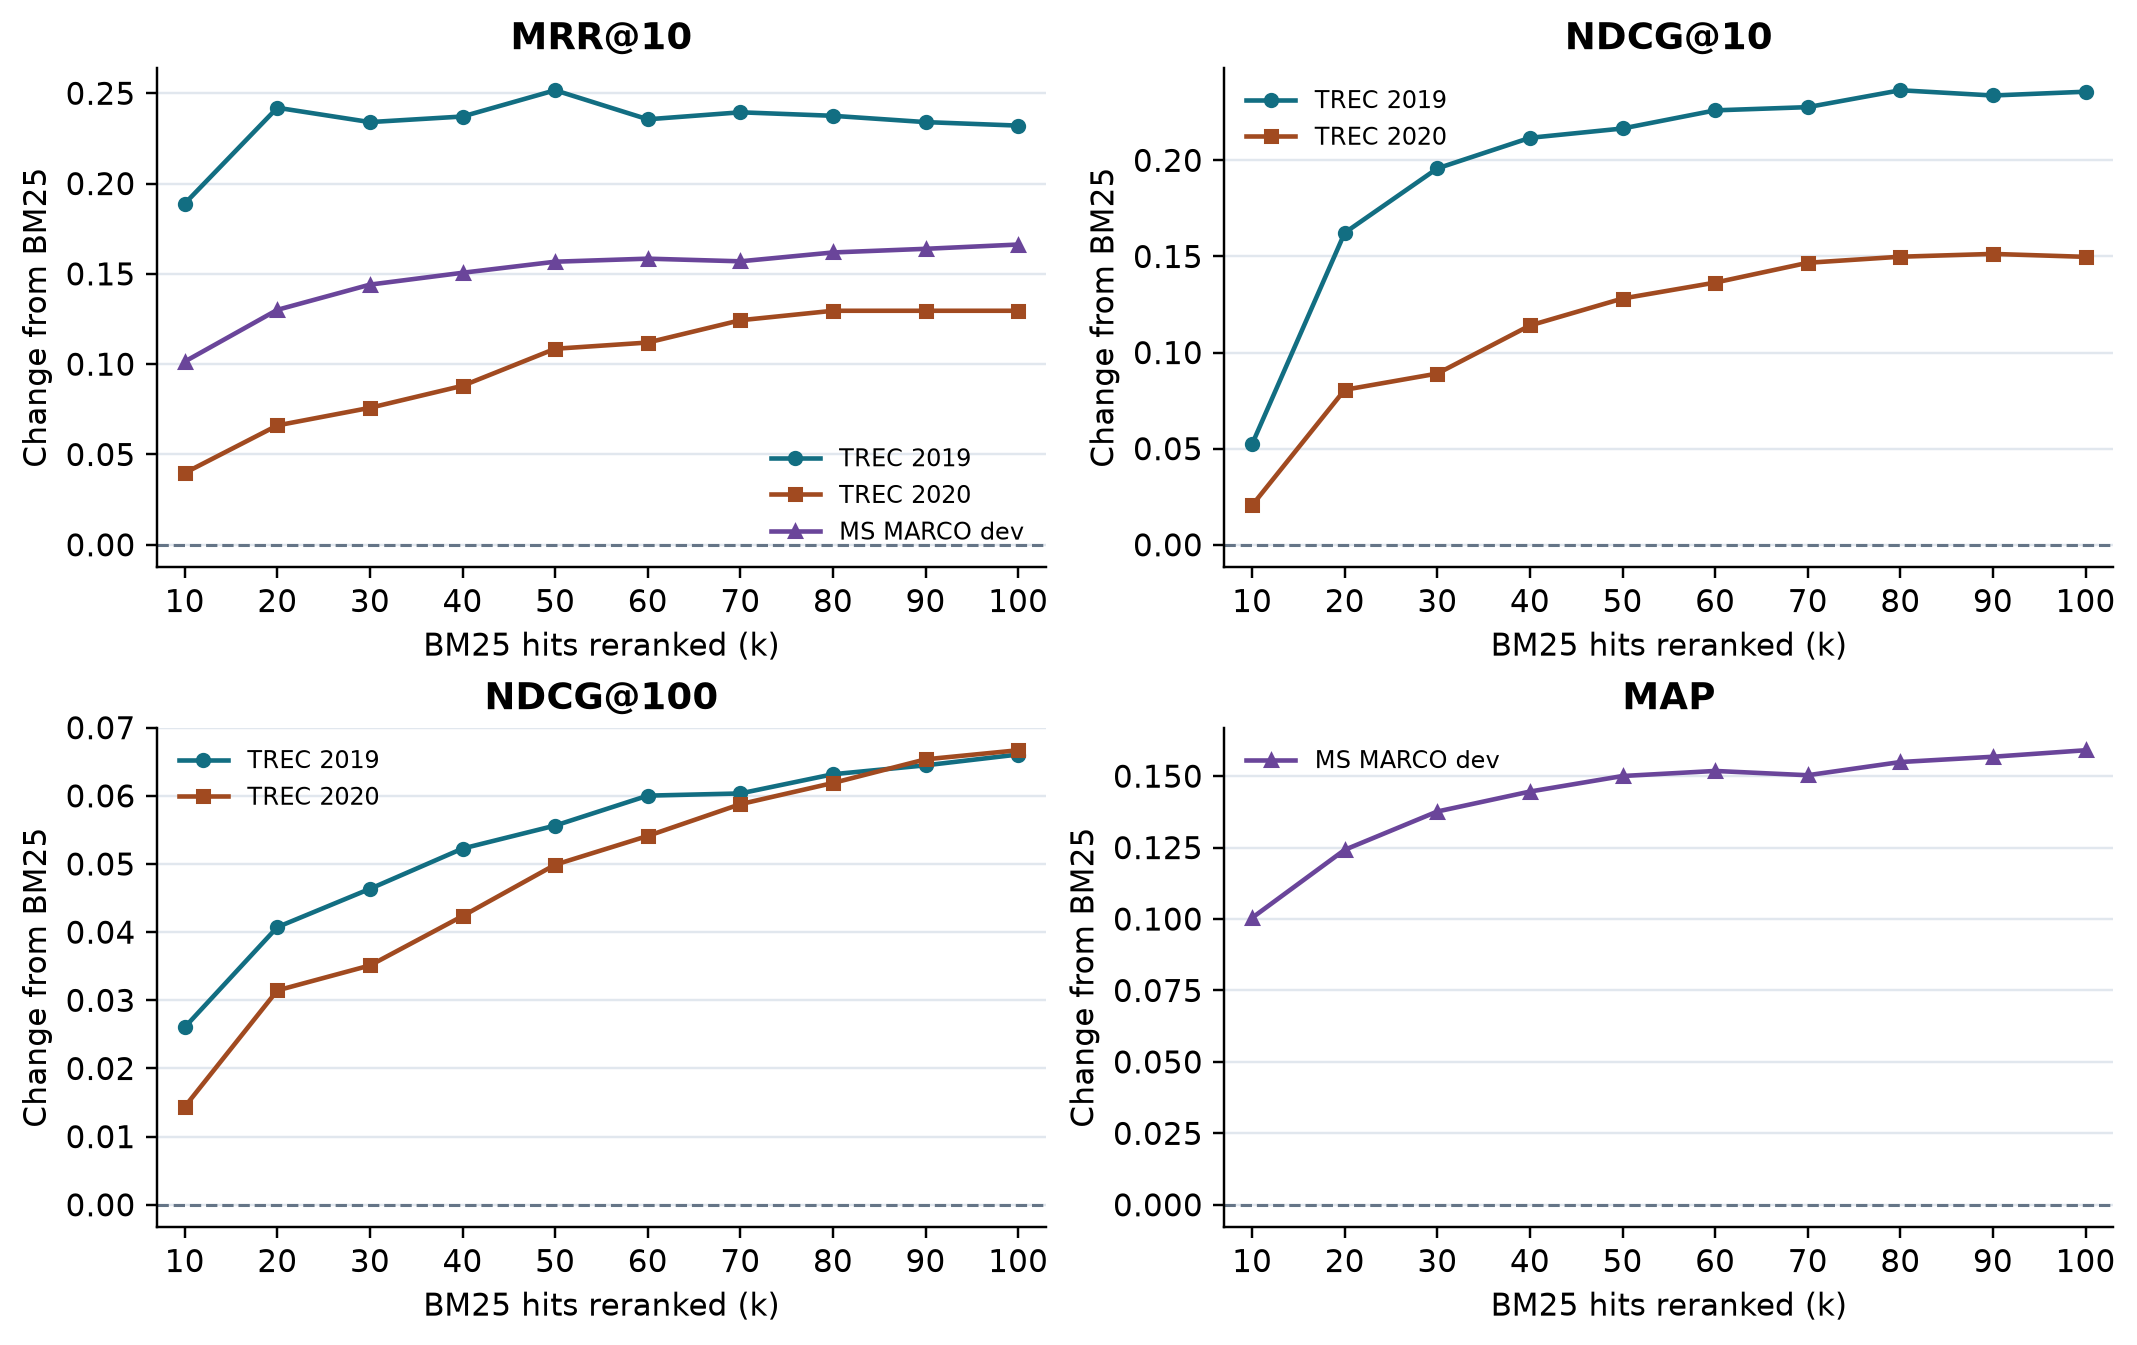
\includegraphics[width=\linewidth]{reranking-cutoff.png}
\caption{Average change from BM25 by reranking depth. The dashed line is zero change.}
\label{fig:depth}
\end{figure}

On TREC 2019, MRR@10 gained 0.1889 at $k=10$ and peaked at a gain of 0.2517 at $k=50$. It fell to a gain of 0.2321 at $k=100$, while NDCG@100 reached a gain of 0.0661. MRR@10 depends on where the first relevant hit lands. A larger reranking window can uncover a good passage from deeper in the list, and it can also push an existing relevant hit lower. NDCG@100 responds to changes throughout the first 100 ranks, so the two curves can move differently.

On TREC 2020 the MRR@10 gain rose from 0.0397 to 0.1296 between $k=10$ and $k=100$. Dev MAP gains rose from 0.1004 to 0.1591 over the same range. Every tested depth improved the mean of each plotted metric. The largest gains occurred at different depths, and the peaks describe results on these judged queries. Choosing a depth for a new collection would require separate validation.

\newpage

\section{Quality by query length}
We counted contiguous alphanumeric tokens, including repeats. Each point averages queries of exactly that length. Figures~\ref{fig:trec-length} and \ref{fig:dev-length} use the full reranker with up to 1,000 candidates. Hollow markers indicate fewer than five queries.

\begin{figure}[H]
\centering
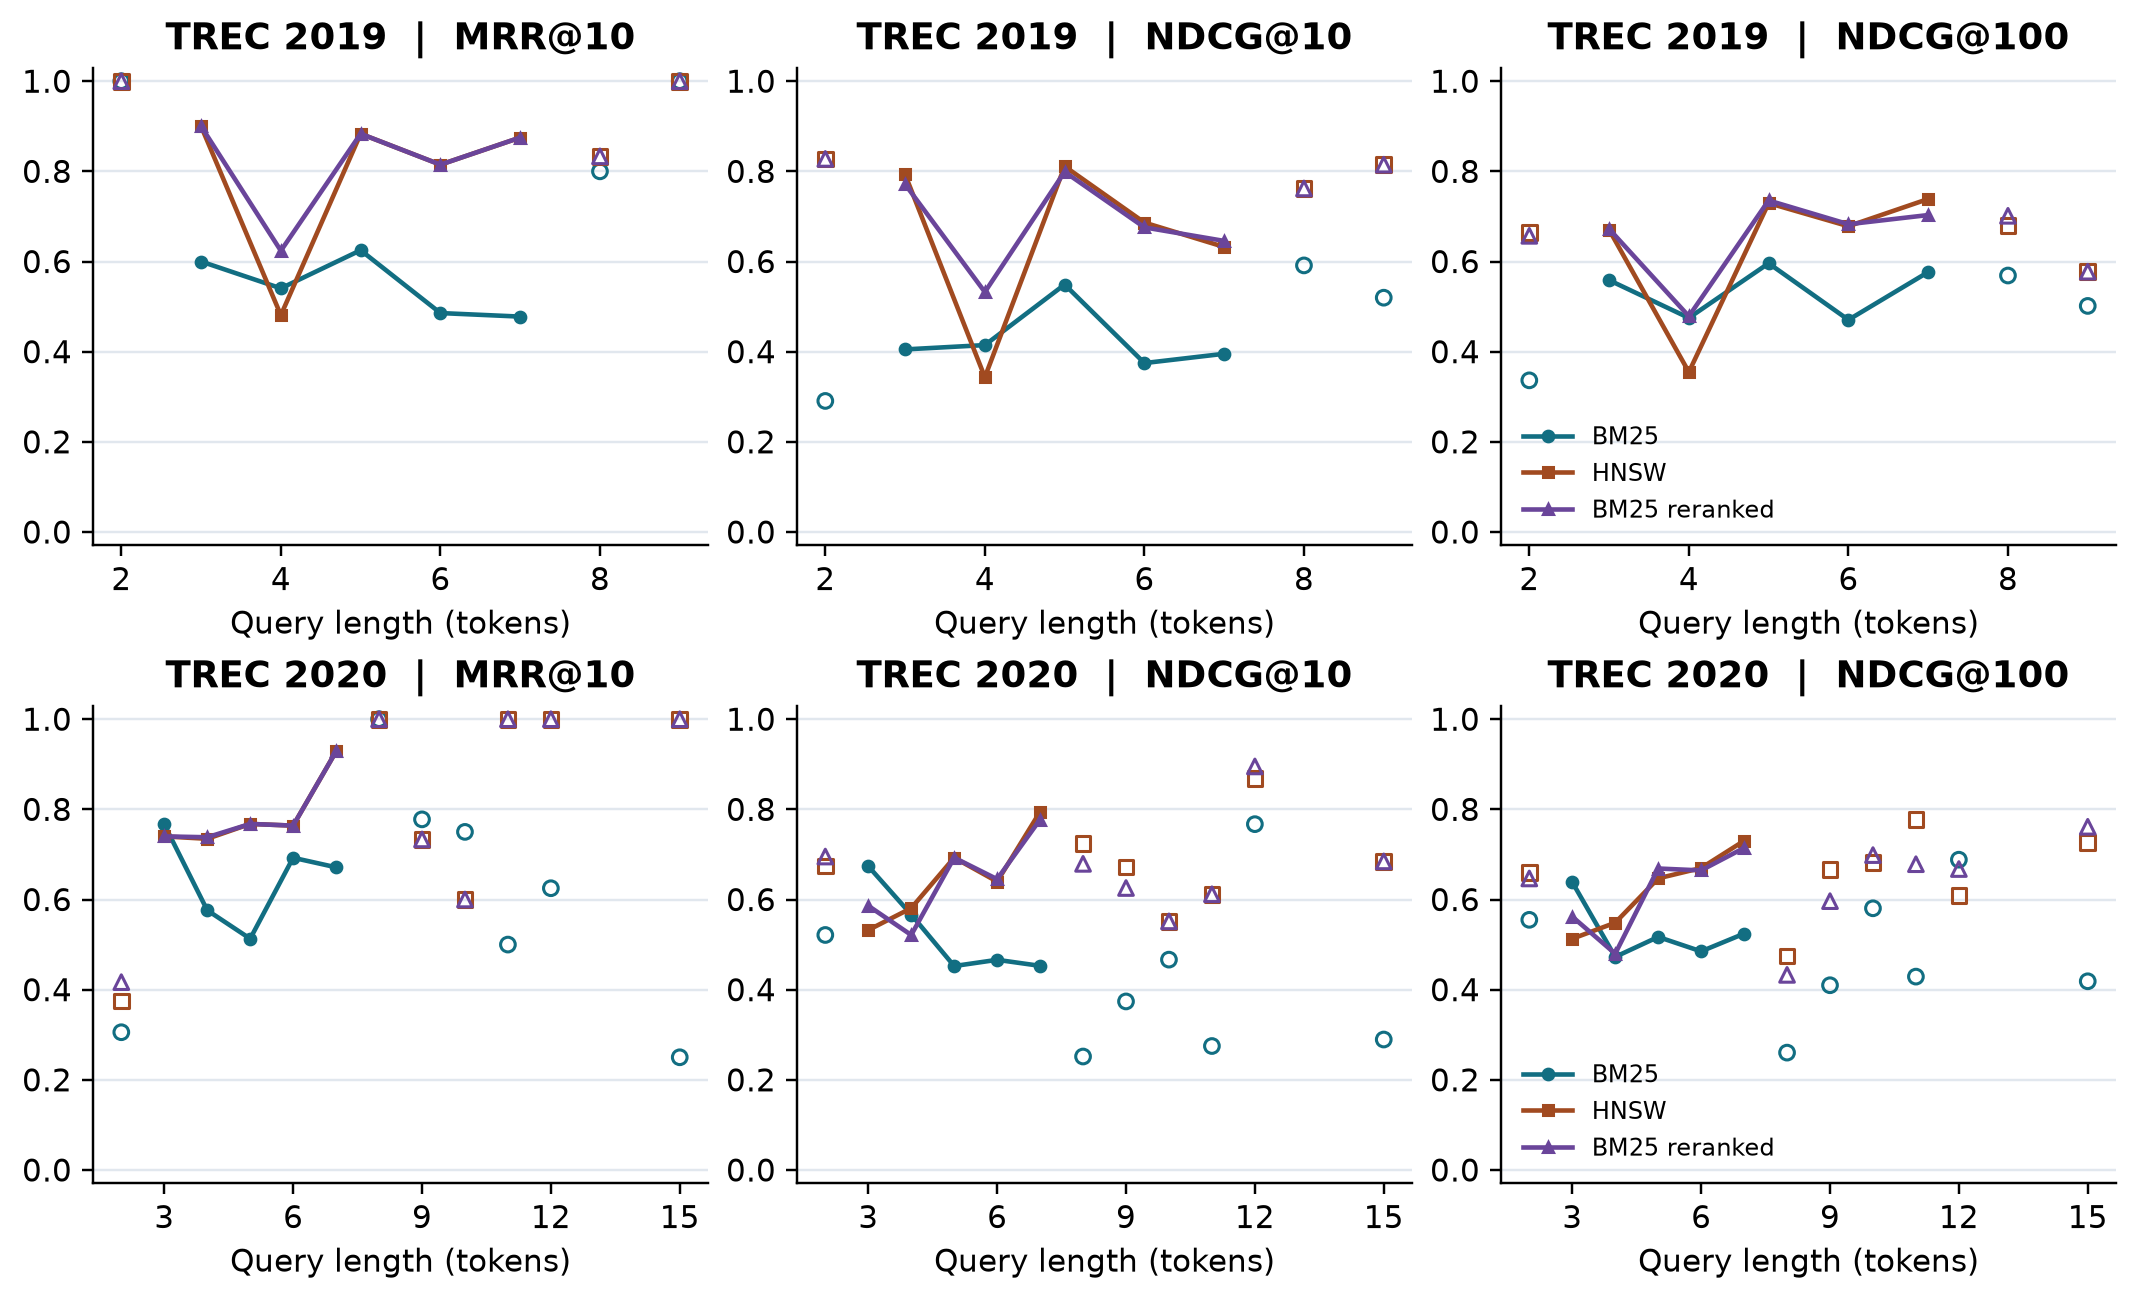
\includegraphics[width=0.98\linewidth]{query-length-trec.png}
\caption{Mean MRR@10 and NDCG by query length for TREC 2019 and TREC 2020.}
\label{fig:trec-length}
\end{figure}
\begin{figure}[H]
\centering
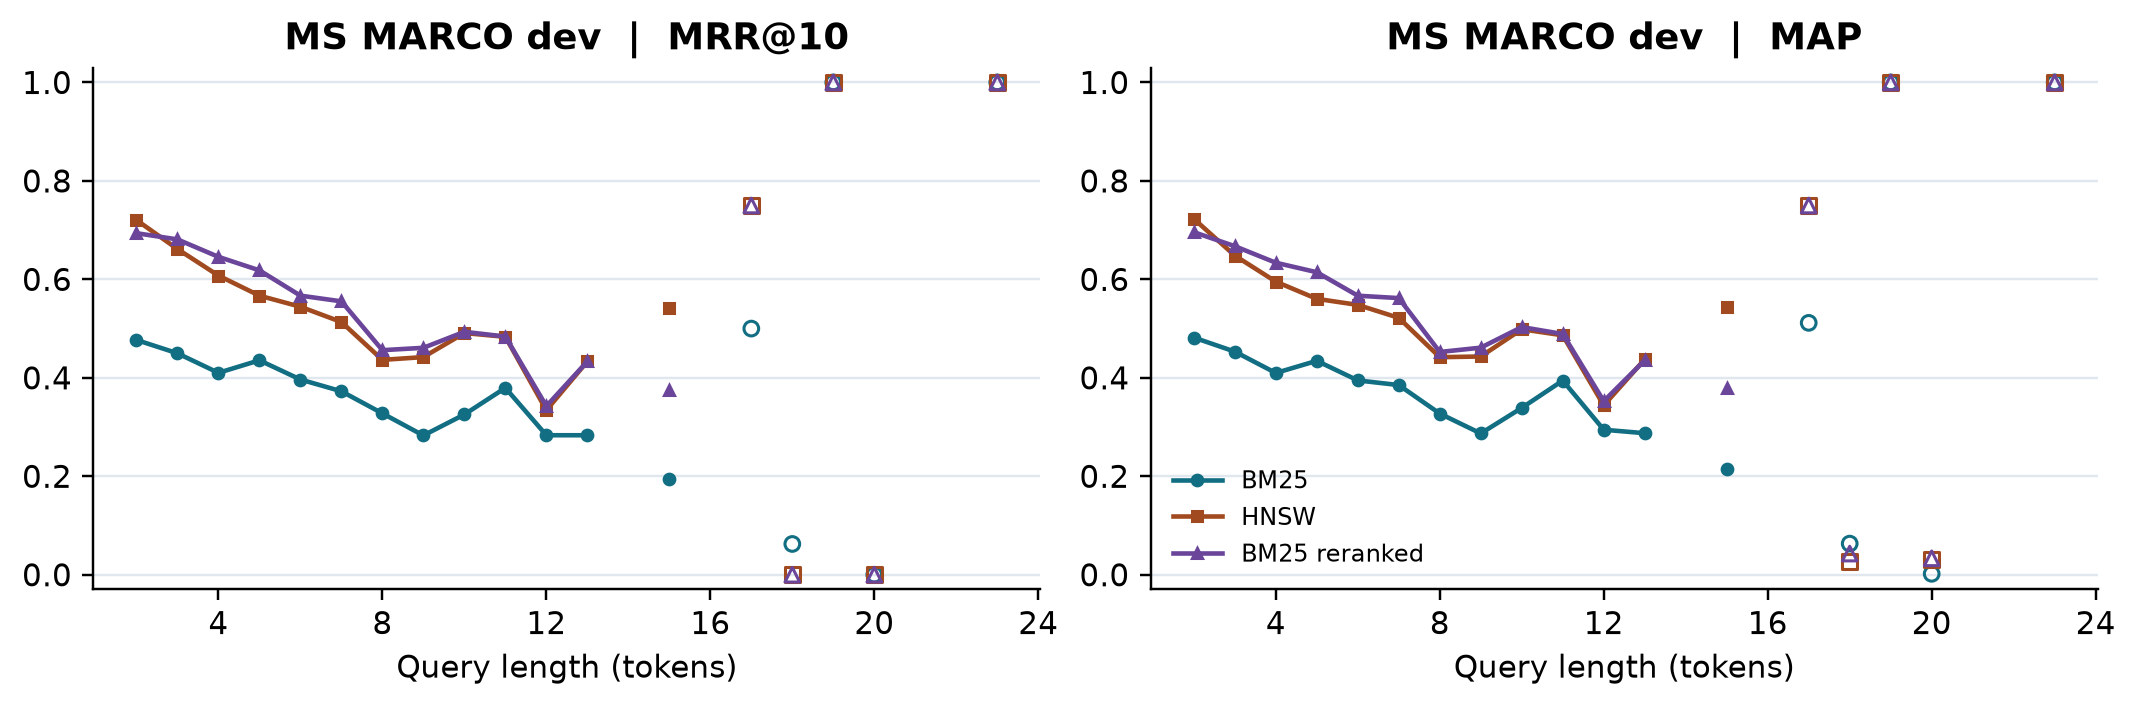
\includegraphics[width=0.98\linewidth]{query-length-dev.png}
\caption{Mean MRR@10 and MAP by query length on MS MARCO dev.}
\label{fig:dev-length}
\end{figure}

On dev, mean MRR@10 was lower for the 92 eight-token queries than for the 169 four-token queries. The change was 0.410 to 0.328 for BM25, 0.608 to 0.436 for HNSW, and 0.646 to 0.456 for reranking. The TREC curves vary more across lengths. For example, the TREC 2020 eight-token point represents one query and the five-token point represents 11. These are comparisons across groups of different queries. Topic, wording, and the number of judged relevant passages can vary along with length.

\newpage
\section{Efficiency}
We used one Apple Silicon Mac with 10 logical CPUs, Python 3.12.12, and FAISS 1.16.0. We timed one build per index and excluded compilation. We measured all systems on the same 43 TREC 2019 queries at depth 1,000. Batch results are medians of three fresh processes after warmup, with trial order rotated. Batch wall time includes startup, loading, retrieval, and writing. Memory is peak resident set size (RSS).

\begin{table}[H]
\centering\small
\caption{Index construction on one million passages.}
\label{tab:build}
\begin{tabular}{@{}lrrr@{}}
\toprule
Index & Time (s) & Peak RSS (MiB) & Size (MiB)\\
\midrule
BM25 & 7.09 & 1,476.4 & 126.4\\
HNSW & 71.04 & 2,271.4 & 1,549.3\\
\bottomrule
\end{tabular}
\end{table}

\begin{table}[H]
\centering\small
\caption{Median batch cost for 43 queries.}
\label{tab:batch}
\begin{tabular}{@{}lrr@{}}
\toprule
Query path & Time (s) & Peak RSS (MiB)\\
\midrule
BM25 & 1.471 & 148.8\\
HNSW & 0.908 & 1,546.1\\
Rerank saved candidates & 0.768 & 1,217.6\\
BM25 and reranking & 2.329 & 1,217.6\\
\bottomrule
\end{tabular}
\end{table}

HNSW was fastest for the full 43-query batch, with a roughly tenfold increase in query RSS and a roughly twelvefold increase in persisted index size over BM25 (Tables~\ref{tab:build} and \ref{tab:batch}). Reranking reused BM25 and 927.0 MiB of supplied embedding files. Its median vector and ID-map loading time was 0.591 seconds, and scoring, sorting, and writing took 0.066 seconds. The full pipeline ran BM25 and reranking sequentially, so its peak RSS is the larger of the two process peaks.

Query embeddings were supplied. The reported wall times capture the batch workflow on this machine. Single-query latency and cold-cache performance require separate measurements. Quality comes from the persisted runs, and efficiency comes from fresh builds with the same settings.


\subsection{What the cost includes}
HNSW took about ten times as long to build in this experiment, but its measured batch time was 38 percent lower than BM25's. A workload that frequently rebuilds the index pays the higher build cost more often. A workload that serves many batches from one index can reuse that build, assuming enough memory is available to load it.

The saved-candidate reranking step took 0.768 seconds at the median. That number is useful if a candidate file already exists. For a fresh query batch the comparable time is 2.329 seconds because the pipeline must first run BM25. The 0.066 seconds spent processing and writing the reranked list was small relative to the 0.591 seconds spent loading vectors and ID maps. A process that caches the embeddings across batches could amortize this setup, but the benchmark measured fresh processes.

Peak RSS is the largest amount of resident memory observed during a measured process. For the sequential pipeline, we take the larger of the BM25 and reranking process peaks within each trial. Disk size reports the persisted BM25 and HNSW indexes. Reranking needs the BM25 index and access to the supplied embedding files. These values describe the tested implementation and machine.

\newpage

\section{Conclusion}
Both approaches that use embeddings improved every reported aggregate metric over BM25. Reranking was strongest on TREC 2019 and dev, while direct HNSW retrieval led on TREC 2020 recall and graded ranking. BM25 had the smallest index and lowest query memory. HNSW returned the 43-query batch fastest with higher construction, storage, and memory costs. The full reranking pipeline added work after BM25, with most of the measured reranking stage spent loading embeddings.

The experiments use one collection, one supplied embedding model, and one HNSW configuration. The small TREC splits make query-level counts and sample sizes useful context for the means. The benchmark covers a warmed batch workload and leaves single-query latency and other hardware settings for separate measurement.
\section{Reproduction}
From the repository root, run the commands below with the supplied MS MARCO files in \path{data/ms_marco/} and the full passage collection at \path{data/data_set.tsv}. The three retrieval commands produce all splits by default. For the 43-query demo, add \texttt{--split eval.one} to the BM25, HNSW search, reranking, and evaluation commands.

{\footnotesize
\begin{verbatim}
uv venv --python 3.12 .venv
uv pip install --python .venv/bin/python faiss-cpu==1.16.0 \
  h5py==3.16.0 numpy==2.5.4 matplotlib==3.11.2
source .venv/bin/activate
python scripts/1_prepare_ps3_subset.py
python scripts/2_build_ps3_bm25.py
python scripts/3_run_ps3_bm25.py
python scripts/4_run_ps3_hnsw.py build
python scripts/4_run_ps3_hnsw.py search
python scripts/5_run_ps3_rerank.py
python scripts/6_evaluate_ps3.py
python scripts/7_benchmark_ps3.py
python scripts/8_analyze_ps3.py
\end{verbatim}
}

\begin{thebibliography}{9}\footnotesize
\setlength{\itemsep}{1pt}
\setlength{\parskip}{0pt}
\bibitem{bm25}
S.~Robertson and H.~Zaragoza.
\newblock The probabilistic relevance framework: BM25 and beyond.
\newblock \href{https://doi.org/10.1561/1500000019}{\emph{Foundations and Trends in Information Retrieval}}, 2009.

\bibitem{hnsw}
Y.~A. Malkov and D.~A. Yashunin.
\newblock Efficient and robust approximate nearest neighbor search using hierarchical navigable small world graphs.
\newblock \href{https://arxiv.org/abs/1603.09320}{arXiv:1603.09320}, 2018.

\bibitem{faiss}
FAISS contributors.
\newblock \href{https://github.com/facebookresearch/faiss/wiki/Faiss-indexes}{FAISS indexes and HNSW parameters}.

\bibitem{trec19}
NIST.
\newblock \href{https://trec.nist.gov/data/deep2019.html}{TREC 2019 Deep Learning Track passage judgments}.

\bibitem{trec20}
NIST.
\newblock \href{https://trec.nist.gov/data/deep2020.html}{TREC 2020 Deep Learning Track passage judgments}.
\end{thebibliography}



\end{document}
